\documentclass{scrartcl}
\usepackage{pgfplots}
\usepackage{graphicx}
\usepackage[left=1cm, right=1cm, top=1cm, bottom=3cm]{geometry}
\renewcommand{\thesection}{\Roman{section}-}
\renewcommand{\thesubsection}{\Roman{section}-\arabic{subsection}}

\usepackage{titlesec}
\titlelabel{\thetitle\quad}

\begin{document}

	\title{\vspace{-2cm}Compte-rendu de travaux pratiques de chimie}
	\subtitle{Dosages par conductimétrie}
	\author{Benjamin Loison (MPSI 1)}
	\date{16 mars 2019}
	\maketitle

  \setcounter{section}{2}
	\section{Dosages par conductimétrie}
		\subsection{Dosage d'une solution d'acide chlorhydrique par la soude}
	
			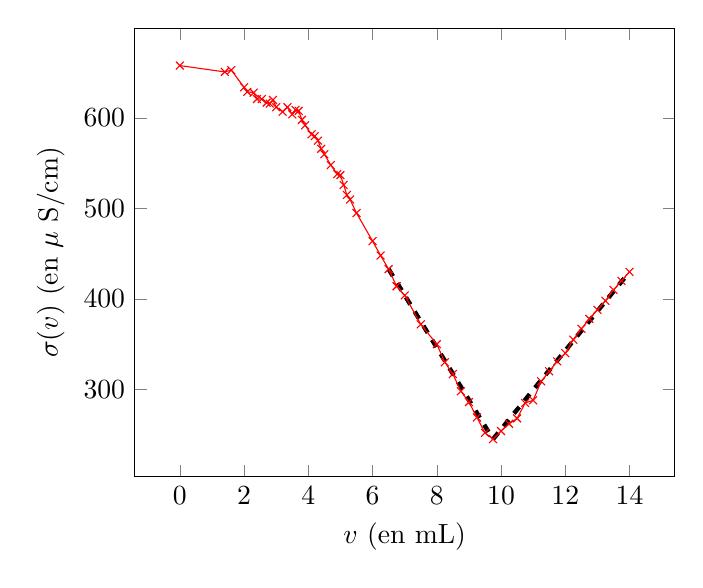
\begin{tikzpicture}
			\begin{axis}[
				xlabel=$v$ (en mL),
				ylabel=$\sigma(v)$ (en $\mu$ S/cm)]
		  \addplot[color = black, dashed, ultra thick] coordinates {(6.5, 433) (9.75, 245)};
		  \addplot[color = black, dashed, ultra thick] coordinates {(9.75, 245) (14, 430)};
			\addplot[color = red, mark = x] coordinates {
				(0, 658)
				(1.4, 651)
				(1.6, 653)
				(2, 634)
				(2.1, 629)
				(2.3, 628)
				(2.4, 621)
				(2.55, 621)
				(2.7, 617)
				(2.8, 616)
				(2.9, 620)
				(3, 612)
				(3.2, 607)
				(3.35, 612)
				(3.5, 604)
				(3.6, 609)
				(3.7, 608)
				(3.8, 598)
				(3.9, 592)
				(4.1, 582)
				(4.2, 580)
				(4.3, 575)
				(4.4, 566)
				(4.5, 560)
				(4.7, 548)
				(4.9, 538)
				(5, 537)
				(5.1, 526)
				(5.2, 515)
				(5.3, 510)
				(5.5, 495)
				(6, 464)
				(6.25, 448)
				(6.5, 433)
				(6.75, 414)
				(6.75, 414)
				(7, 404)
				(7.5, 372)
				(8, 350)
				(8.25, 330)
				(8.5, 317)
				(8.75, 298)
				(9, 286)
				(9.25, 269)
				(9.5, 252)
				(9.75, 245)
				(10, 254)
				(10.25, 262)
				(10.5, 268)
				(10.75, 285)
				(11, 288)
				(11.25, 309)
				(11.5, 320)
				(11.75, 331)
				(12, 340)
				(12.25, 355)
				(12.5, 367)
				(12.75, 378)
				(13, 388)
				(13.25, 398)
				(13.5, 410)
				(13.75, 420)
				(14, 430)
			};
			\end{axis}
		\end{tikzpicture}
			
		\noindent\underline{Interprétation qualitative:}\\\\
		Aucune valeur relative à la constante de la cellule n'est disponible sur ce conductimètre.\\
		Dans un premier temps lorsque l'on introduit $n$ moles de soude, celles-ci consomment $n$ moles de $H_3O^+$ de l'acide chlorhydrique ($H_3O^+$, $Cl^-$). Car l'hydroxyde de sodium (soude) en solution a pour formule ($Na^+$, $OH^-$). Ainsi la conductivité baisse car on a $\Lambda_{H_3O^+}^0 \gg \Lambda_{HO^-} \gg \Lambda_{Na^+}^0$. Il en résulte que les ions sodium et chlorure sont spectateurs et la conductivité des ions sodium est négligeable devant celle de $H_3O^+$ et $HO^-$. Donc globallement la conductivité baisse.\\
		En linéarisant le graphique on détermine le volume équivalent $v_e = 9.45$ mL.\\
		On a d'après le tableau d'avancement relatif à l'équation de réaction: $c_a = \frac{c_{NaOH} * v_e}{v_{HCl}} = \frac{0.1 * 9.75 * 10^{-3}}{10 * 10^{-3}}$ = 0.0975 mol.L$^{-1}$ soit environ 0.1 mol.L$^{-1}$. % sure ? make tableau d'avancement
		La pipette jaugée à deux traits de 10 mL (de classe A) a une tolérance de $\pm$ 0.050 mL et la burette graduée de dosage de 25 mL (de classe A) avec une graduation au 0.1 mL a une tolérance de $\pm$ 0.05 mL.\\
		On néglige l'approximation d'eau distillée versée pour négliger les effets de dilutions.\\
		On considère que les concentrations des deux espèces chimiques, celle de dosage et celle à doser, sont approximatives à 1 \% près.\\
		L'incertitude globale sur la concentration de l'espèce à doser $c_a$ est donnée par: $\Delta c_a = \sqrt{\frac{\Delta c_{NaOH} * \Delta v_e}{\Delta v_{HCl}}}$ avec $\Delta X$ l'incertitude sur les quantitées intermédiaires.\\ % sure ?
		Application numérique: $\Delta c_a = \sqrt{\frac{0.001 * 0.05}{0.050}}$ = 0.032 mol.L$^{-1}$.\\% sure ? special frac for converting 0.05 into a concentration error and integrate in 0.001 with a plus ?
		 %?! Donc $c_a = 0.0975 \pm 0.032$ mol.L$^{-1}$. Donc l'intervalle de confiance à 95 \% de $c_a$ est: [$c_a - 2\Delta c_a; c_a + 2\Delta c_a$] soit [0.0335; 0.1615].
		\\
		
		\noindent\underline{Interprétation théorique:}\\\\
		
		% TODO
		
		\subsection{Dosage d'une solution d'acide acétique (ou éthanoïque) par la soude}
		
			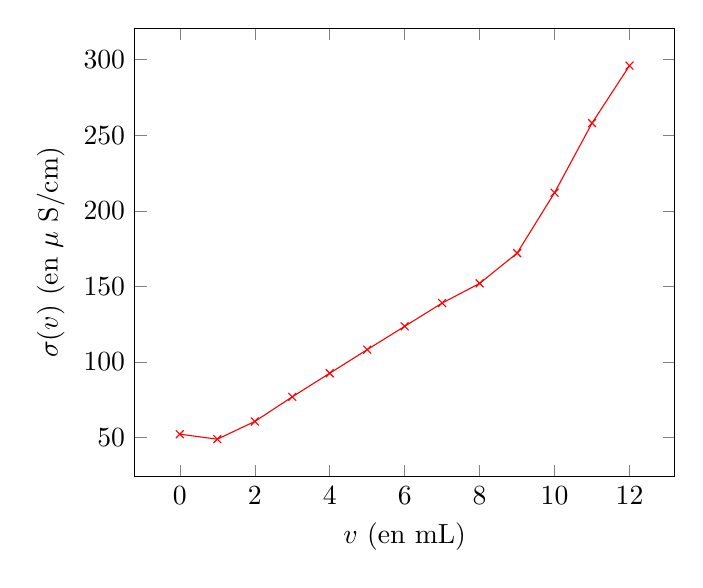
\begin{tikzpicture}
			\begin{axis}[
				xlabel=$v$ (en mL),
				ylabel=$\sigma(v)$ (en $\mu$ S/cm)] % better data ?
			\addplot[color = red, mark = x] coordinates {
				(0, 52.3)
				(1, 49.0)
				(2, 60.7)
				(3, 77.0)
				(4, 92.6)
				(5, 108.2)
				(6, 123.6)
				(7, 139.0)
				(8, 152)
				(9, 172)
				(10, 212)
				(11, 258)
				(12, 296)
			};
			\end{axis}
		\end{tikzpicture}
		
		\subsection{Dosage d'une solution d'acide acétique (ou éthanoïque) par la soude, en présence d'ammoniac}
		
			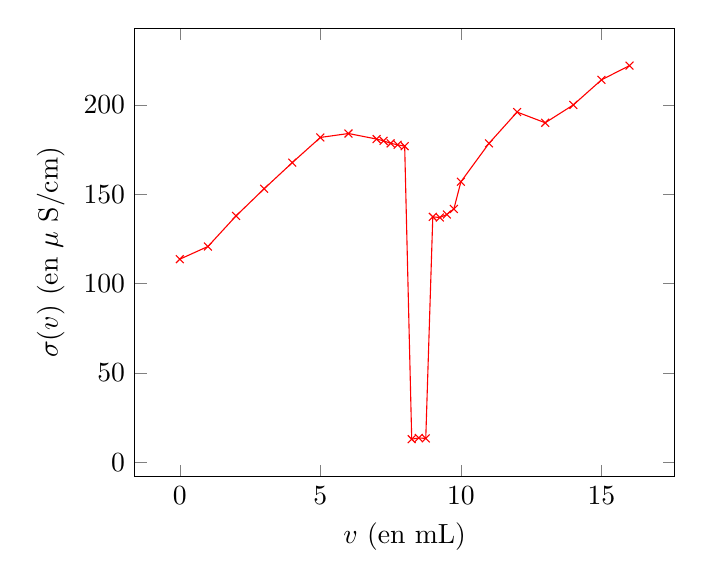
\begin{tikzpicture}
			\begin{axis}[
				xlabel=$v$ (en mL),
				ylabel=$\sigma(v)$ (en $\mu$ S/cm)] % better data ?
			\addplot[color = red, mark = x] coordinates {
				(0, 113.7)
				(1, 120.8)
				(2, 137.9)
				(3, 153.1)
				(4, 167.7)
				(5, 181.8)
				(6, 184.0)
				(7, 180.9)
				(7.25, 179.9)
				(7.5, 178.5)
				(7.75, 177.7)
				(8, 176.9)
				(8.25, 13)
				(8.5, 13.7)
				(8.75, 13.43)
				(9, 137.4)
				(9.25, 137)
				(9.5, 138.7)
				(9.75, 141.8)
				(10, 157)
				(11, 178.5)
				(12, 196.0)
				(13, 190)
				(14, 200)
				(15, 214)
				(16, 222)
			};
			\end{axis}
		\end{tikzpicture}
		
		Les valeurs relevés entre 7.5 et 10 mL sont erronées.
			
\end{document}